\chapter{Electrons Are Not Little Planets Orbiting the Nucleus}

\begin{kaichang}
Old streets in many cities still have a traditional kind of streetlight. At dusk, it first glows dull red, then gradually brightens to orange-yellow over several minutes, bathing the street as though in orange soda. This is a \textbf{sodium lamp}, containing a little sodium vapor and inert gas.

Here is a worthwhile puzzle. Neon signs can glow red, blue, green, purple, and countless other colors, but sodium lamps always have the same orange-yellow. Is the manufacturer lazy? No. The color is neither paint nor tinted glass: it grows from inside sodium atoms. Sodium can emit only that color, and only that color, like someone able to sing just a few fixed notes.

Now consider holiday fireworks: who dyes them red, green, gold, or blue? Write down a guess. By the end of this chapter, you will find strict lodging rules for energy floors behind the colors. Those rules form the foundation of our next great map, the periodic table.
\end{kaichang}

\section{Take Light Apart and Look}

Color can be taken apart. Sunlight through a triangular prism spreads into a continuous rainbow, with every color from red to violet and no gaps. Newton used this to show that white light mixes all colors. Similar continuous colors appear on the back of a CD and on soap bubbles.

Now change the source. Pass sodium-lamp light through a prism, or the more precise spectroscope of a physics laboratory. What do you expect? Not a rainbow, but isolated bright lines: two closely spaced yellow lines are especially dazzling, with almost blackness elsewhere. Red-glowing neon gas likewise gives separated lines, not a continuous band. Every gas and element has its own pattern, identical whether measured in Beijing or Paris, a lamp tube or a star.

This cornered nineteenth-century scientists: \textbf{every element has a fixed spectral fingerprint}. Light emerges from inside atoms. Fixed fingerprints imply fixed, discontinuous internal structures. Invisible atoms were mailing us their interiors through light.

These fingerprints work around you today. In old fluorescent tubes, mercury vapor emits ultraviolet light, which the wall's phosphor translates into several visible colors mixed as white. Banknote detectors excite fluorescent security marks with ultraviolet; their emitted colors are atomic fingerprints too. Spectral glasses sold outside planetariums distinguish sodium lamps from LEDs when aimed at streetlights: their apparently white lights have entirely different patterns when separated. Color is one of the cheapest and quickest ways to distinguish substances.

An even more familiar version exists. Add a little sodium salt to a flame and it immediately glows bright yellow, the same yellow as the streetlight. You can safely try this flame-color phenomenon once at home.

\begin{shiyan}
\textbf{Observe Table Salt's Flame Color} (An adult's presence is recommended.)

\textbf{Materials}: a small spoonful of salt, a little less than half a cup of water, a cotton swab or clean stainless-steel spoon, and a candle or a small gas-stove flame.

\textbf{Procedure}: Dissolve salt in water to make concentrated brine. Light the candle and observe its original flame color, mostly pale blue with yellow near the wick. Soak the swab in brine and hold its wet tip at the flame's upper edge without touching the wick. Watch the color change. Rewet several times and repeat.

\textbf{What to observe}: (1) What color does the brine-soaked swab give the flame? (2) Is it pure yellow or a mixture? (3) Does the color disappear immediately when you remove the swab?

\textbf{Safety}: Wet the swab before approaching the flame, and dip it in water if it catches fire. Do not sprinkle dry salt into flames. Extinguish the candle afterward and put matches away. Use only table salt; do not try other powders.

Your bright yellow, sodium streetlights, and gold in fireworks come from the same spectral lines of the same atom. Salt is sodium chloride, \chem{NaCl}, and the yellow belongs to sodium, not chlorine. Potassium chloride instead gives pale violet. The flame is a temporary atomic broadcasting station, announcing sodium's identity in color.
\end{shiyan}

\section{The Planetary Model Hits Two Walls}

Chapter 7 described Rutherford's gold-foil discovery: almost all atomic mass and all positive charge occupy a tiny nucleus, with electrons outside. An obvious picture follows: electrons circle the nucleus like planets around the Sun. This planetary model is easy to understand and draw, and still adorns countless textbook covers.

Unfortunately, it is decisively wrong. Two walls block its way.

The first is electromagnetism. Nineteenth-century physics established that accelerating charges emit electromagnetic waves and lose energy. Circular motion is acceleration because direction changes continuously. An electron truly orbiting like a planet should glow and lose energy as it circles, shrinking its orbit until it spirals into the nucleus. Calculated collapse time is about $10^{-10}$ seconds: such an atom would not survive one hundred-millionth of a second. Yet this book and all its atoms exist stably in your hands. That is the model's fatal crime: it predicts atoms that cannot stand.

The second wall is the spectrum. Planets can occupy orbits of any radius, allowing continuous energy changes and therefore continuous emitted light. Actual measurements instead show discrete bright lines. If electrons could have arbitrary energies, spectral fingerprints should not exist.

The contradiction is plain: stable atoms and fixed, separated spectral lines. Together, they announce that electron energies cannot vary continuously but \textbf{can take only certain particular values}. Like a staircase, you can stand on one step or another, but not suspended midway between them.

\section{Electrons Occupy Energy Floors, Not Orbits}

In 1913, Bohr imposed a bold new rule on hydrogen: its electron could occupy only particular energy levels, meaning allowed energy values, without radiating while there. Only a jump between levels absorbs or emits a photon, with energy exactly equal to the difference.

This immediately explained everything. Why discrete spectral lines? Fixed level differences allow only particular photon energies, hence particular colors. Why different fingerprints? Different nuclear positive charges produce different level arrangements, like buildings with different stair heights. Why no collapse? There is a lowest level, the \textbf{ground state}, the lowest-energy lodging floor. An electron there has nowhere lower to jump, so nowhere to collapse.

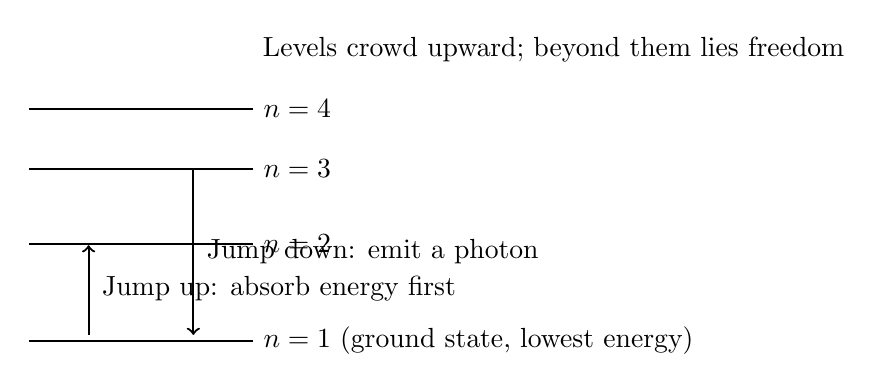
\begin{tikzpicture}[scale=0.95]
\draw[thick] (0,0) -- (3,0) node[right] {$n=1$ (ground state, lowest energy)};
\draw[thick] (0,1.3) -- (3,1.3) node[right] {$n=2$};
\draw[thick] (0,2.3) -- (3,2.3) node[right] {$n=3$};
\draw[thick] (0,3.1) -- (3,3.1) node[right] {$n=4$};
\node[right] at (3,3.9) {Levels crowd upward; beyond them lies freedom};
\draw[->,thick] (2.2,2.3) -- (2.2,0.08);
\node[right] at (2.25,1.2) {Jump down: emit a photon};
\draw[->,thick] (0.8,0.08) -- (0.8,1.28);
\node[right] at (0.85,0.7) {Jump up: absorb energy first};
\end{tikzpicture}

This drawing is a human representation. Horizontal lines indicate allowed energies, not lines on which electrons physically stand. Energy levels are \textbf{marks on an energy scale}, not floors at geographic locations.

Jumping between upper and lower floors sounds like particle acrobatics. The real difficulty comes next: when an electron occupies a level, where exactly is it?

\section{An Electron Cloud: A Probability Map, Not a Motion Blur}

Quantum mechanics, developed by Schrödinger, Heisenberg, and others in the 1920s, gave an uncomfortable answer that no experiment has overturned: \textbf{between measurements, an electron has neither a definite position nor a trajectory}.

Read that slowly. It does not mean electrons move too fast to follow, or that better instruments will someday pinpoint them. It means the question ``at which point is the electron now?'' has no answer before measurement. Quantum mechanics calculates the \textbf{probability} of finding it at a position outside the nucleus: whether nearer positions or particular directions are more probable. Those predictions can be extraordinarily precise, agreeing with experiment to many decimal places.

The word orbital survived, but with a completely new meaning. An orbital is not a route but \textbf{the shape of a probability distribution}, a three-dimensional map of where an electron is likely to be found. Draw denser dots for higher probabilities and sparser dots for lower ones, and you obtain an \textbf{electron cloud}:

\begin{itemize}[itemsep=2pt]
\item \textbf{s orbitals}: spherical. Electrons are most likely near a certain distance from the nucleus, with no preferred direction.
\item \textbf{p orbitals}: dumbbell-shaped, with two lobes on opposite sides of the nucleus. Three p orbitals align along the mutually perpendicular $x$, $y$, and $z$ directions.
\item \textbf{d and f orbitals}: more complicated, with more petals. At school level, knowing they exist is enough.
\end{itemize}

These shapes outline probability maps, not hard shells, balloons, or regions occupied by electrons. Drawings often enclose a boundary where, say, there is a ninety-percent probability of finding the electron. It is a reference line like a forecast rain boundary, not a wall.

How should we understand probability? Imagine a superinstrument that repeatedly photographs the position of hydrogen's ground-state electron. Every snapshot contains one solitary point: an electron is never a little cloud in a single appearance. Take ten thousand photographs and superimpose their points. Dense areas form dark regions, sparse areas remain scattered, and the whole makes a spherical pattern around the nucleus. An electron cloud resembles this composite. \textbf{The cloud is a statistical result of countless position measurements, not an electron spread into a cloud in one observation, and certainly not a blurred trail from rapid motion.}

\begin{wuqu}
``The electron cloud is a blur from an electron orbiting so fast that its path merges, like spinning fan blades becoming a disk.'' This misconception is widespread because it seems intuitive, but it is fundamentally wrong.

Three rebuttals help. First, every electron detection finds a definite point, never a short stretched trajectory. If a trajectory existed, sufficiently high energy should reveal a swept trace, but none appears. Second, motion blur cannot explain stability: a truly accelerating, orbiting electron would radiate and spiral into the nucleus under electromagnetic laws, collapsing the atom in about $10^{-10}$ seconds as calculated earlier. The electron avoids collapse precisely because it does not perform that circular motion. Third, ground-state hydrogen's cloud is a spherically symmetric, time-independent pattern. Why would a running electron's blur remain forever uniform and unchanged?

The proper picture is that there is no electron trajectory to leave a trail. The cloud depicts probabilities of finding it at different positions, and probability itself has that shape. Accepting this is uncomfortable, but a century of experiments has voted for the uncomfortable picture.
\end{wuqu}

Incidentally, the planetary model's true failure goes deeper than collapse. Quantum mechanics says an electron confined to atomic dimensions cannot have a definite velocity and orbit. This is a natural law, Heisenberg's uncertainty principle, not a technological limitation. The more tightly it stays home inside the atom, the less definite its state of motion. A definite circular orbit would require definite position and velocity simultaneously, which nature refuses.

\section{The Energy Hotel's Lodging Rules}

Many-electron atoms have dozens of residents to accommodate, and nature enforces strict hotel rules. You need not memorize them; understand three principles.

\textbf{Rule one: floors and room types.} Electron energy depends mainly on principal quantum number $n$, with $n=1,2,3,\cdots$ identifying floors. Higher numbers generally mean higher energy and greater average distance from the nucleus. Each floor has room types s, p, d, and f, the differently shaped probability maps. Floor 1 has only s (1s); floor 2 adds p (2s and 2p); floor 3 adds d; floor 4 adds f.

\textbf{Rule two: at most two occupants per room, back to back.} Besides position and energy, electrons possess an intrinsic property called \textbf{spin}, resembling a tiny top. It is not literal spinning, only behavior with two orientations. The \textbf{Pauli exclusion principle} permits at most two electrons per orbital, with opposite spins. Thus 1s holds 2, the three 2p orbitals together hold 6, and floor 2 holds 8 overall. This produces shell capacities $2,8,18,32$.

\textbf{Rule three: choose cheaper rooms first, and occupy equivalent rooms singly before sharing.} Electrons fill lowest-energy orbitals first, the \textbf{Aufbau principle}: 1s before 2s, 2s before 2p. Equal-energy rooms of one type, such as three 2p orbitals, first receive one electron each with parallel spins, then begin pairing only when necessary. This is \textbf{Hund's rule}. Imagine strangers taking separate benches until all are occupied, then agreeing to sit together. Behind the analogy, like charges repel and separation lowers energy.

Now the symbols enter. Writing floor, room type, and occupancy makes an electron lodging register: hydrogen is \chem{1s^1}, helium \chem{1s^2}, filling the first shell; carbon \chem{1s^2 2s^2 2p^2}; sodium \chem{1s^2 2s^2 2p^6 3s^1}. Sodium's first two shells are full like neon's, while one lonely electron occupies shell 3. That solitary electron determines almost its entire personality. Chapter 10 unfolds how these personalities arrange elements into the periodic table.

\textbf{Rules have exceptions, and we must not hide them.} Aufbau would predict chromium as \chem{3d^4 4s^2}, but measurements give \chem{3d^5 4s^1}; copper would be \chem{3d^9 4s^2}, but is \chem{3d^{10} 4s^1}. Half-full (5) and full (10) d rooms are especially favorable, so a 4s electron moves house. This does not abolish the rule; it reminds us that lodging rules approximate an energy account involving every electron--electron repulsion. Rules with honest exceptions are far more reliable science than perfect but false mnemonics.

\begin{qiaoliang}
A photon's color determines its energy: $E = hc/\lambda$, where $\lambda$ is wavelength and $h$ and $c$ are constants. Shorter wavelengths toward blue and violet mean higher photon energy.

Calculate a real example. The sodium lamp's two yellow lines have wavelengths near \ud{589}{nm}, or $5.89\times10^{-7}$ meters. The formula gives about $3.4\times10^{-19}$ joules per photon, a tiny amount. At the other end of the scale, a \ud{100}{W} sodium lamp converting all electrical power to this yellow light would emit each second
\[100 \div (3.4\times10^{-19}) \approx 3\times10^{20}\ \text{photons}.\]
Three sextillion photons per second, each emitted when a sodium electron returns from 3p to 3s. Atoms are tiny, but their energy differences made into light can illuminate a whole street.

The reverse use is even more revealing: \textbf{measure light's color to infer an atom's internal energy-level difference}. Spectroscopy becomes a telescope into atoms because light reports level spacing without cutting an atom open.
\end{qiaoliang}

\section{An Element First Discovered on the Sun}

\begin{zhengju}
The fingerprint idea was not invented on a whim. Its history is an interlocking chain of evidence.

In 1814, the German lens maker Fraunhofer was testing prisms, passing sunlight through a narrow slit before a prism, when he unexpectedly saw hundreds of fine \textbf{dark lines} across the rainbow. Particular colors had vanished on the way to Earth. He recorded their positions but could not explain them. The mystery persisted over forty years.

In 1859, Heidelberg's chemist Bunsen and physicist Kirchhoff solved it. Bunsen's modified gas burner, today's laboratory Bunsen burner, produced a hot, nearly colorless flame. Each salt placed in it yielded unmistakable elemental bright-line patterns. Kirchhoff then made the crucial test: strong light passed through sodium vapor before entering the prism produced dark lines exactly where sodium's bright lines belonged. Atoms both emit and absorb their characteristic colors. Solar dark lines are fingerprints of light intercepted by atoms in the Sun's outer gas layers. Spectroscopy could identify not only terrestrial elements but the composition of a star over ninety million kilometers away. A recent declaration that humanity could never know stellar chemistry was overturned almost as soon as it was made.

The method immediately became an element detector. In 1860, Bunsen found two unfamiliar sky-blue lines in mineral-water residue and announced cesium, named from Latin for sky blue. The following year brought rubidium, dark red. A bolder event came in 1868: observing solar prominences during an eclipse, the French astronomer Janssen found a yellow line matching neither sodium nor any known element. The British astronomer Lockyer asserted that it belonged to a new solar element not yet found on Earth, helium, from Greek for Sun. Many colleagues thought a new element based on one line absurd. Twenty-seven years later, in 1895, Ramsay found the same line in gas released while treating uranium ore. Helium was discovered on the Sun before being found on Earth.

One last why remained: why those particular wavelengths? Bohr's 1913 level model correctly calculated hydrogen lines, and 1920s quantum mechanics incorporated many-electron atoms. Every link---dark lines, flame colors, predictions of new elements, energy-level theory---could be tested and overturned by later investigators, and all survived. That is the proper meaning of how scientists know.
\end{zhengju}

\section{The Limits of This Picture}

The electron-cloud model is extraordinarily successful, but understanding its boundaries is part of understanding it.

First, Bohr's hybrid of energy levels and orbits works precisely only for hydrogen. Many-electron atoms require quantum-mechanical approximations; electron repulsions create tens of thousands of terms for computers. When saying floors, remember this only approximates $n$. In many-electron atoms, s, p, and d within one shell have different energies; 4s even fills before 3d, behind the chromium and copper exceptions.

Second, spherical and dumbbell cloud shapes strictly map one electron's probability. Treating them as individual rooms for every electron in a large atom is extremely useful, but mutual jostling makes the true picture more complicated than separate rooms.

Third, probability is not a last resort forced on us by ignorance. Some proposed definite but unknown electron trajectories, so-called hidden variables. Bell-inequality experiments in the later twentieth century decisively excluded a major, natural class of such explanations. Electron fuzziness belongs to nature rather than our ignorance. Increasingly precise experiments continue testing this boundary.

Fourth, clouds concern only the region outside nuclei. Protons, neutrons, and radioactivity follow Chapter 8's different rules; electrons negotiating between atoms to form chemical bonds begin in Chapter 17.

\section{Back to the Orange-Yellow Streetlight}

We can now answer the opening question. In a sodium lamp, current lifts the outer electron from 3s to 3p. On returning, it emits a photon whose energy corresponds exactly to \ud{589}{nm}, the yellow to which human eyes are most sensitive. This color cannot change because it is set by the height difference between two internal steps. Fixed steps mean fixed color. Changing the element is the only way to change the lamp's color: neon glows red-orange, argon blue-violet, xenon white. A street of neon signs is an exhibition of atomic energy levels.

Fireworks work likewise. Strontium salts burn vivid red, barium grass-green, copper deep blue, while dazzling gold usually comes from our familiar sodium. The flame you personally lit, streetlights, fireworks, and stellar spectra are different scenes of the same physical law.

Go deeper: every color corresponds to a definite level difference, and the entire staircase follows from lodging rules. Their most astonishing product, as the next chapter shows, is a table rather than colors. Why do its widths run 2, 8, 8, 18? Why do elements in one column have matching personalities? Why did Mendeleev dare leave gaps and predict undiscovered elements? In Chapter 10, we unfold the electron lodging register and see it grow into the periodic table's oddly shaped city.

\begin{tiaozhan}
Bohr's finest achievement was calculating all hydrogen energy levels with one formula: $E_n = -13.6/n^2$, in electronvolts eV, with $n=1,2,3,\cdots$. The minus sign indicates an electron bound to the nucleus, below the energy of freedom.

Try predicting a spectral line. A jump from $n=3$ to $n=2$ emits a photon of energy
\[\Delta E = 13.6\times\left(\frac{1}{2^2}-\frac{1}{3^2}\right) = 13.6\times\frac{5}{36} \approx 1.89\ \text{eV}.\]
Convert to wavelength, using 1 eV corresponding to approximately \ud{1240}{nm}: $1240 \div 1.89 \approx 656$ nm, a red line. This is hydrogen's most conspicuous red spectral line, H$\alpha$, used by telescopes to identify cosmic hydrogen clouds. A formula on paper predicts stellar colors. If interested, calculate $n=4$ to $n=2$ and $n=5$ to $n=2$ too, and compare their colors with a hydrogen spectrum. Skipping this passage does not interrupt the main story.
\end{tiaozhan}

\section*{Try It Yourself}

\begin{sikaoti}
\item Draw hydrogen levels $n=1$ through $n=4$, following this chapter's staircase. Show downward paths from $n=3$ directly to $n=1$, and from $n=3$ via $n=2$ to $n=1$. Which step emits the highest-energy photon? Is its light bluer or redder? Note that lines represent energy values, not electron positions in space.
\item Write oxygen's 8-electron and magnesium's 12-electron configurations using floor, room type, and occupancy. How many electrons does each outermost shell contain?
\item A student draws a 1s electron as a dashed circle around the nucleus and calls it the electron's path. Identify two mistakes and correct the drawing. (Hint: use scattered dots, with denser dots indicating greater probability of finding the electron.)
\item To make purple fireworks, a worker mixes red strontium salts and blue copper salts. Explain from energy levels why this might work. Could heating sodium salts more strongly turn their yellow light blue? Why?
\item Helium was discovered on the Sun 27 years before Earth. What justified assigning a line to an unseen element? If someone called it instrumental error, what experiment could settle the dispute?
\end{sikaoti}
